\documentclass[11pt, english]{article}
        \usepackage{geometry}
                \geometry{
                        a4paper,total={210mm,297mm},
                        tmargin=40.8mm,
                        bmargin=40.8mm,
                        lmargin=32.6mm,
                        rmargin=32.6mm,
                }

        \usepackage{titlesec}
                \titleformat{\section}
                        {\normalfont\fontsize{18}{16}\bfseries}{\thesection}{0.5em}{}
                \titleformat{\subsection}
                        {\normalfont\fontsize{14}{16}\bfseries}{\thesubsection}{1em}{}
                \titleformat{\subsubsection}
                        {\normalfont\fontsize{11}{16}\bfseries}{\thesubsubsection}{1em}{}

        \usepackage{longtable}
        \usepackage{multirow}

        \usepackage[labelfont=bf,textfont=bf,font=small,skip=8pt]{caption}

        \setlength{\parindent}{0pt}
        \renewcommand{\baselinestretch}{1.25}
        \usepackage{setspace}

        \usepackage{amsmath}
        \usepackage{amssymb}

	\usepackage{graphicx}

\begin{document}

\pagenumbering{gobble}

        \title{\textsc{AG217 Portfolio Management \& Security Analysis\\ Coursework Assignment}}
        \author{\textsc{Lewis Britton}}
        \date{\textsc{Academic Year 2018/2019}}
        \maketitle

\newpage

\pagenumbering{roman}

        \renewcommand{\contentsname}{Table of Contents}

        \tableofcontents

\newpage

\pagenumbering{arabic}

\section{Problem Set Questions}

	\subsection{Question 1}

	First, the monthly excess returns for Hong Kong were calculated by subtracting the risk-free, Treasury Bill, returns from the market returns for Hong Kong, in an (N,1) matrix. The mean of these excess returns was then calculated (Table 1), which shows a 0.93\% average excess return in the Hong Kong market. As can be seen (Table 1), volatility is clear at 7.2\%, by the standard deviation value.\\

	Furthermore, a conclusion must be reached based on the sampling variation of the excess return estimate and its performance against the risk-free Treasury Bills. This was done by reaching the standard error value of 0.41\% (Table 1), showing significant variation from the mean value. This value then allowed for analysis of hypotheses. Here, this examines whether market return (R$\mathrm{_m}$) will equal zero by making risk-free rate (R$\mathrm{_f}$) hypothetically equal to zero – that is, null – and would therefore yield an answer equal to zero, inferring Rm is zero.  For the Hong Kong data, the hypotheses are as follows: H$_0$ referring to the average excess market return of Hong Kong being equal to zero and H$\mathrm{_A}$ referring to the average return not being equal to zero.\\

	From this equation, we observed a t-statistic of 2.2943 (Table 1). This further gave a p-value of 0.0224 which allowed for evaluation of the probability of observing the t-statistic, as opposed to comparing the actual t-statistic to the critical values of the t-distribution. This p-value is $<$ 0.05, the significance level, which means we reject the null hypothesis (H$_0$) in favour of the alternative hypothesis (H$\mathrm{_A}$) at this 5\% significance level.\\

	This analysis means that there is strong evidence to show that the mean excess market return of Hong Kong (R$\mathrm{_m}$) is not 0, supported by the fact that the h-value is 1 (Table 1). Through rejection of the null hypothesis here, we see that the average excess returns for Hong Kong differ from zero due to a real difference in value and not simply just experimental error or chance. Further inferring that the return found in the Hong Kong Stock Exchange differs significantly from that of US Treasury Bills. Hence, the fact that the p-value is $<$ 0.05 and the t-statistic is positive show that R$\mathrm{_m}$ is significantly positive which means that return on the Hong Kong market heavily outweighs risk free returns on the Treasury Bills. 

	The observed 95\% confidence interval of (0.0013, 0.0174) or, 0.13\%, 1.74\% (Table 1) means that there is a 95\% probability of the population mean lying within this range. This also highlights large sampling error when observing R$\mathrm{_m}$. Overall, all of the above further indicates the Hong Kong market provides greater returns on average than investments in US Treasury Bills.

\newpage

	\subsection{Question 2}

	After compiling a matrix of the whole market’s excess returns, mean values can be calculated within each country’s market. These display the average expected performance and act as a baseline for comparing markets. It can be seen that Finland’s market, at 10.1\%, shows the highest mean, historic return value and therefore can initially be expected to be most profitable, solely based on past returns. Where the USA’s market is shown to be least profitable at only 0.47\% on average. However, Finland’s market actually offers the highest standard deviation value, at 8.47\%, which means it has been observed to deviate the most from its mean value, immediately removing it from the most reliable investment due to high risk. On the other end, it happens that the USA actually holds the smallest standard deviation meaning that even though it is the least profitable, based on past performance, it is also the least risky. Therefore, making an index in it a better option for, perhaps, inexperienced or longer-term investors. For the average investor however, it is important to find something in the middle. That makes Australia’s market most appealing in this sense. This being due to its reasonable mean excess return at 0.75\%, which is above average – when comparing the ten countries – and, its standard deviation of 5.95\%, which is just around average – when comparing all ten countries.\\

	When observing correlation coefficients, it is important to identify the lowest value as it is important to create diversity in a portfolio. Meaning, you don’t want to invest in portfolios where everything moves in a positively correlated direction – in the same direction as one another. This increases risk massively. By having negatively correlated assets in a portfolio, there is greater probability of offsetting loss thus, reducing risk. Here, we will take our most reliable market form before – Australia, based on risk and return, and observe which country’s markets it correlates the least amount to, to form a possible optimal portfolio. Australia is seen to correlate least to Finland but, we can discard that due to earlier observations. Therefore, we take Spain due to its promising combination of return, deviation and correlation to Australia.

\newpage

	\subsection{Question 3}

	To proceed in analysing the excess returns for the given ten countries, Mean Variance Analysis must be sought in context, through Markowitz’s idea of efficiency, to analyse a portfolio constructed of ten assets (Markowitz, 1952). That is, the ten countries’ markets.\\

	After observing the Efficient Frontier, it is important to identify the portfolio with the lowest level of risk, relative to the generated covariance matrix of the excess returns. The most optimal distribution of wealth must be identified – Asset Allocation. This can first be done using the GMV Theory (Markowitz, 1952). Where GMV weights the proportion of investment and this optimal weighting portfolio is mapped on the vertical stationary point of the Efficient frontier. As observed (Table 5), the optimal GMV weights are 3.46\% in Australia, 32.02\% in Belgium, 2.04\% in Canada, -11.79\% in Finland, -1.03\% in France, -19.48\% in Germany, 4.26\% in Hong Kong, -8.13\% in Singapore, 0.63\% in Spain and 99.28\% in the USA’s market (Table 5). Where positive weights represent an expected rise in price – long position. And, negative weights represent where it is best to short sell – short positions (Jacobs, Levy, Markowitz, 2005). This means that the associated markets are expected to fall in value and therefore it would be more profitable to borrow these market assets and return them before the expected price drop, buying back at a later date. Overall however, there is an extreme weight on Spain’s market nearing 100\% and this could look suspicious and unappealing to some investors due to the psychological effects of lack of diversity (Michaud \& Michaud, 2008).\\

	As well as the above, there is an estimation risk within the GMV Theory (Michaud, 1989). Therefore, another method of analysing optimal weights is utilised by looking at the Max Sharpe method where average return expectation is analysed against every unit of volatility (Sharpe, 1994). Here, there is an observation of significant difference. Where this method places short selling only on France, Germany, Singapore and Spain at -0.39\%, -40\%, -55.98\% and -15.78\% weightings, respectively. Where Australia, Belgium, Canada, Finland, Hong Kong and the USA are weighted at 33.44\%, 66.24\%, 6\%, 28.54\%, 70.45\% and 7.48\%, respectively (Table 5). This shows huge deviation in conclusion when looking at investing based on per-unit volatility. As observed, a market which once showed potential on close to a 100\% rating, USA, now shows not even a tenth of that weighting potential. Equally, other values differ in size significantly, some inversely, meaning there is far too much error not accounted and equalised for when observing these methods of analysis (Best \& Grauer, 1991). Further, in these methods of analysis, it is assumed that the expected values and covariance terms are known with absolute certainty, leaving overweighting issues simply regarding low volatility and high return portfolios (Michaud \& Michaud, 2008). Therefore, leaving high estimation error as discussed.

\newpage

	\subsection{Question 4}

	See Table 6.

\newpage

	\subsection{Question 5}

	Due to the discussed estimation error in historically sampled Mean Variance Analysis, cases result in poor out-of-sample performance (Jobson \& Korkie, 1981). Therefore, Jobson \& Korkie utilise the Max Sharpe Analysis to simulate a series of data samples based on the assumption of true expected return and covariance values and the optimal Max Sharpe weights, then simulating a series of results, sample moments, in order to evaluate the overall simulated portfolio in the context of true values. This is known as Multivariate Normal Distribution and is based on expectations for the future – out of sample performance – rather than solely historic data.\\

	When comparing the average out-of-sample Sharpe MV value to the True Sharpe value there is over underperformance observed seen in the Sharpe MV value of 0.1129, compared to the True Sharpe value of 0.1706 (Table 6). However, when comparing the MV Sharpe value to the 1/N Sharpe value of 0.1344, underperformance is observed again meaning the average out-of-sample Sharpe performance of the MV portfolio reflects a less optimal investment when compared to the equally weighted 1/N portfolio. This is reflected in the poor value of the Sharpe MV portfolio outperforming the Sharpe 1/N portfolio. This value is 0.271 meaning only a small proportion of the time, roughly 27\%, the Sharpe MV portfolio will outperform the 1/N portfolio.

\newpage

\section{Problem Set Tables}

	\subsection{Table 1: Hong Kong Excess Return Statistics}

	\begin{center}
                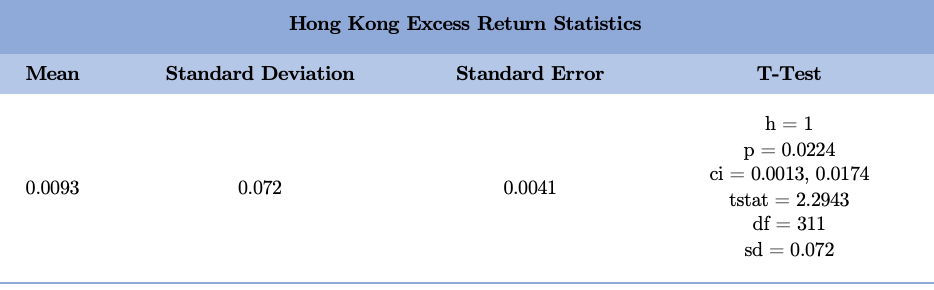
\includegraphics[height=4cm,width=14cm]{AG217-IMG/a.png}
        \end{center}

	This table displays statistics relevant to analysis of Hong Kong’s isolated excess returns. These include the mean average of the returns, the standard deviation (volatility), the standard error and all stats under the t-test. Including the 5\% reject/accept indicator (h), the probability of observing the t-statistic (p), the 95\% confidence interval (ci), the t-stat itself (tstat), the allowed variability of values in the sample within constraint (df) and, the standard deviation (sd). All statistics are displayed in decimal form rather than percentage to remain consistent with the sample data. 

	\subsection{Table 2: Market Sample Means}

	\begin{center}
                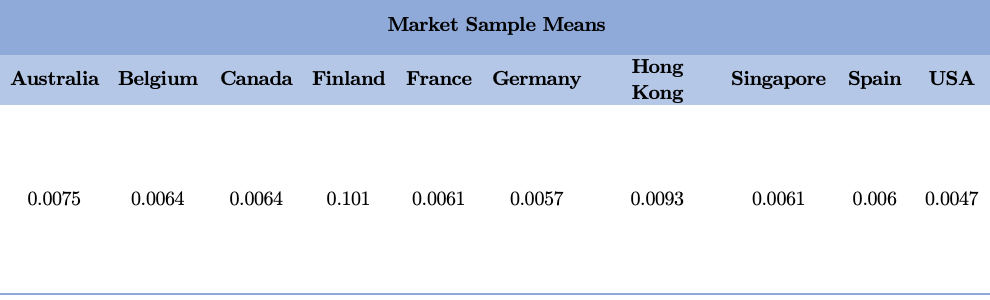
\includegraphics[height=4cm,width=14cm]{AG217-IMG/b.png}    
        \end{center}

	This table displays the mean average values of all ten countries relevant to the analysis. This mean average is based on the excess market returns of the individual countries and thus, indicated a general baseline for comparing market returns to one another. These are presented as real decimal numbers, rather than percentages.

	\subsection{Table 3: Market Standard Deviations}

	\begin{center}
                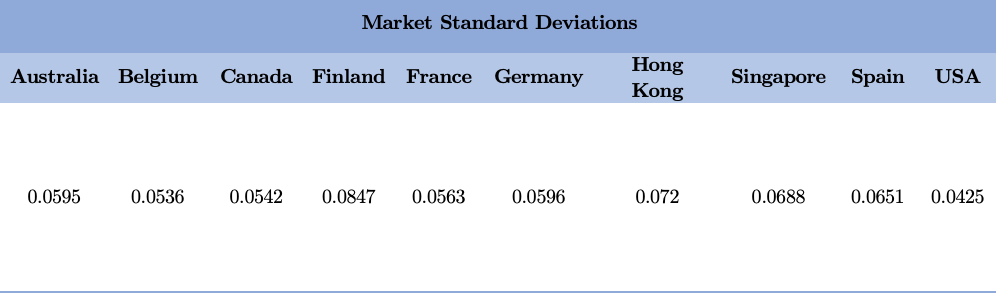
\includegraphics[height=4cm,width=14cm]{AG217-IMG/c.png}    
        \end{center}

	This table displays the standard deviations of the ten countries in question. Thus, showing how much each country’s market returns can deviate from the mean excess return value. As with the mean values, these results are based on the individual excess market returns of each country and are in non-percentage decimal format.

	\subsection{Table 4: Market Correlation Coefficients}

	\begin{center}
                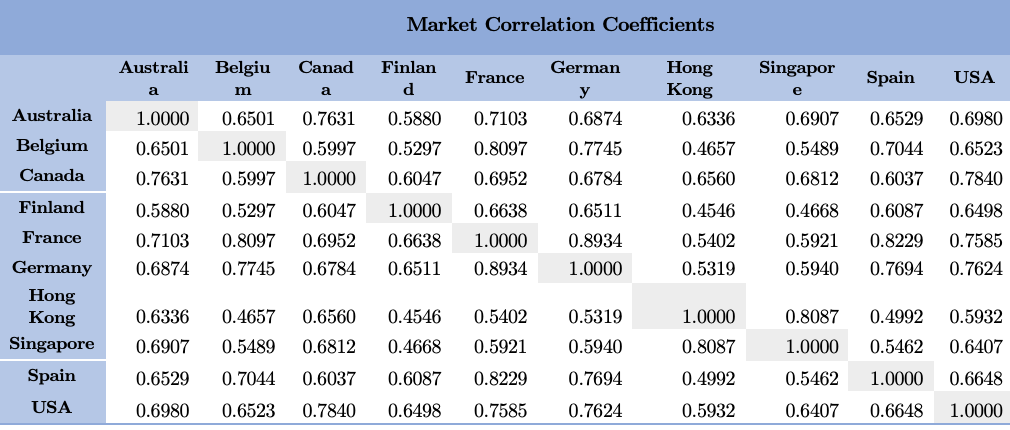
\includegraphics[height=6cm,width=14cm]{AG217-IMG/d.png}    
        \end{center}

	Here, are shown correlation coefficients between each country’s expected return value. Meaning the displayed value reflects how closely each country’s market moves to each other, on a one-to-one level. The closer to one the value, the more similarly the markets move together. Correlations are mirrored, therefore repeated, on either side of the ‘1’ values, due to crossover. The ‘1’ show a country’s correlation with itself.

	\subsection{Table 5: GMV \& Max Sharpe Weighting}
	
	\begin{center}
                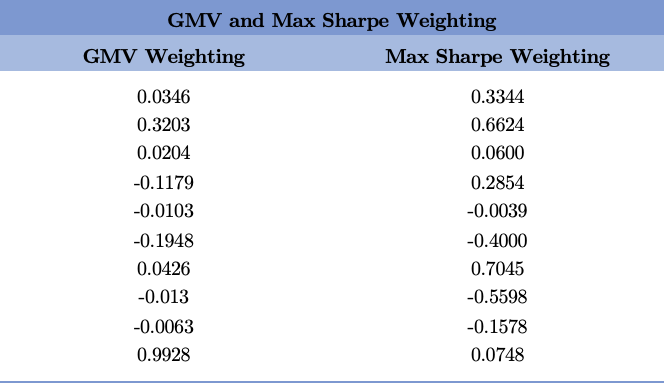
\includegraphics[height=5cm,width=8cm]{AG217-IMG/e.png}    
        \end{center}

	This table shows the GMV and Maximum Sharpe weights for the optimal portfolio of the ten countries’ market, showing the proportion of the portfolio populated by each country. Therefore, the two sums of `GMV Weighting' and `Max Sharpe Weighting' should equal one (100\%). All values are shown in decimal form and were calculated based on covariance (for GMV Weights) and mean expected value (for GMV and Max Sharpe Weights). Optimal weights for both analyses were found subject to only the budget constraint as this is `Unbounded Mean Variance Optimisation'. 

	\subsection{Table 6: Sharpe Testing \& Simulations}

	\begin{center}
                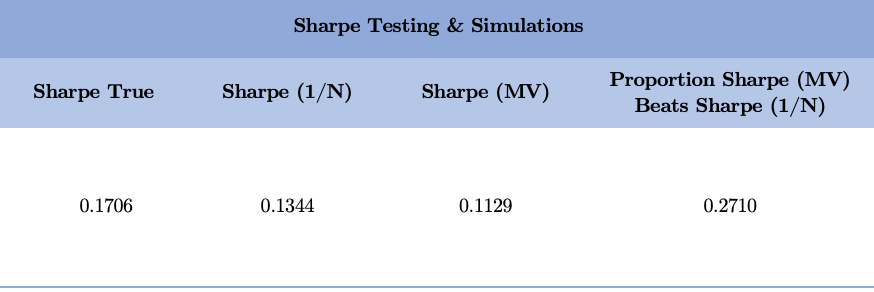
\includegraphics[height=4cm,width=12cm]{AG217-IMG/f.png}    
        \end{center}

	Displayed here is the True Sharpe value, calculated using the true mean excess return and covariance matrix values. Also shown is the 1/N Sharpe value, calculated using the true mean excess return and covariance values. Next, the MV Sharpe value is based on simulating a series of random returns based on the true values of the mean excess returns and covariance matrix. One thousand repetitions took place in this example. A mean value and final covariance matrix of such returns are then produced adapting to equate to optimal weights for the MV portfolio. The optimal weights are finally used to reach a Sharpe MV value taking into account all necessary simulated variables: mean expected return, covariance matrix and weights. Also shown in the table is the proportion to which the Sharpe MV simulated value defeats the equally weighted 1/N Sharpe value. The closer this value to 1, the greater the outperformance.

\newpage

\pagenumbering{Roman}

\section*{Code}

	\begin{center}
                
\includegraphics[height=20cm,width=14cm]{AG217-IMG/g.png}    
        \end{center}

	\begin{center}             
                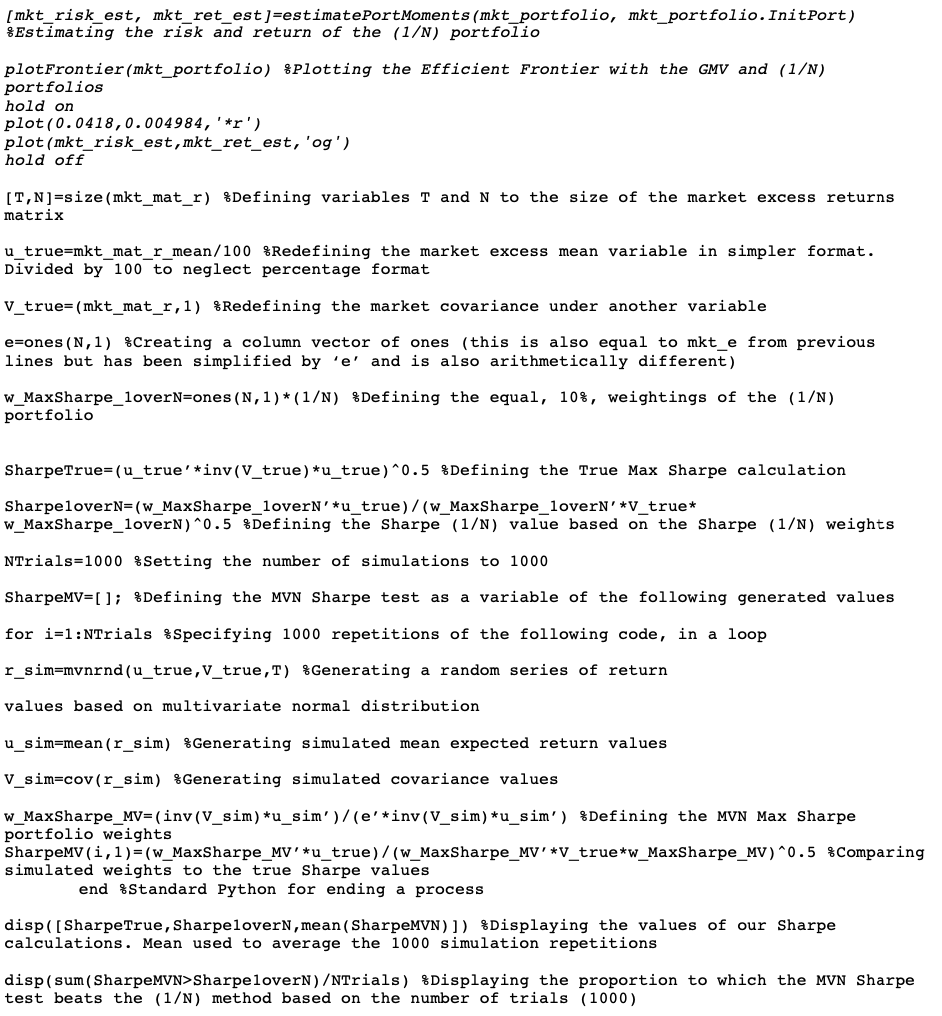
\includegraphics[height=16cm,width=14cm]{AG217-IMG/h.png}    
        \end{center}

\newpage

\renewcommand\refname{Bibliography}

\begin{thebibliography}{9}

	\bibitem{a}
		Best, M., Grauer, R. (1991).
		\textsl{On the Sensitivity of Mean-Variance-Efficient Portfolios to Changes in Asset Means: Some Analytical and Conceptual Results.}
		Review of Financial Studies. Vol. 4.

	\bibitem{b}
		Jacobs, B., Levy, K., Markowitz, H. (2005). 
		\textsl{Portfolio Optimisation with Factors, Scenarios and realistic Short Positions.}
		Operations Research.

	\bibitem{c}
		Jobson, J., Korkie, R. (1981).
		\textsl{Putting Markowitz Theory to Work.}
		The Journal of Portfolio Management.

	\bibitem{d}
		Markowitz, H. (1952).
		\textsl{The Journal of Finance: Portfolio Selection.}
		American Finance Association. Vol. 7, No. 1, Pg. 77-91.

	\bibitem{e}
		Michaud, R.O., Michaud, R.O. (2008).
		\textsl{Efficient Asset Management.}
		Oxford University Press.

	\bibitem{f}
		Michaud, R.O. (1989).
		\textsl{The Markowitz Optimisation Enigma: Is ``Optimized'' Optimal?}
		Financial Analysis Journal. 45, Pg. 31-42.

	\bibitem{g}
		Sharpe, W. (1994).
		\textsl{The Journal of Portfolio Management.}
		Institutional Investor Inc.

\end{thebibliography}

\end{document}
